\chapter{Spectrométrie de masse et spectroscopie atomique}\label{ch:b2:mass-spec-atomic}

Les feux d'artifice sont rouges avec les sels de strontium, verts avec les sels de baryum, jaunes avec
le sodium~: une flamme transforme les atomes en une lumière dont les couleurs les identifient. Un
spectromètre de masse, d'apparence plus modeste, pèse des molécules une à une, les trie selon leurs
isotopes et les brise en fragments dont les masses révèlent comment elles étaient construites. Les deux
techniques répondent à la question «~que contient cet échantillon, et en quelle quantité~?~» à partir de
très petites quantités, la première pour les molécules, la seconde pour les éléments.

\begin{omfigure}
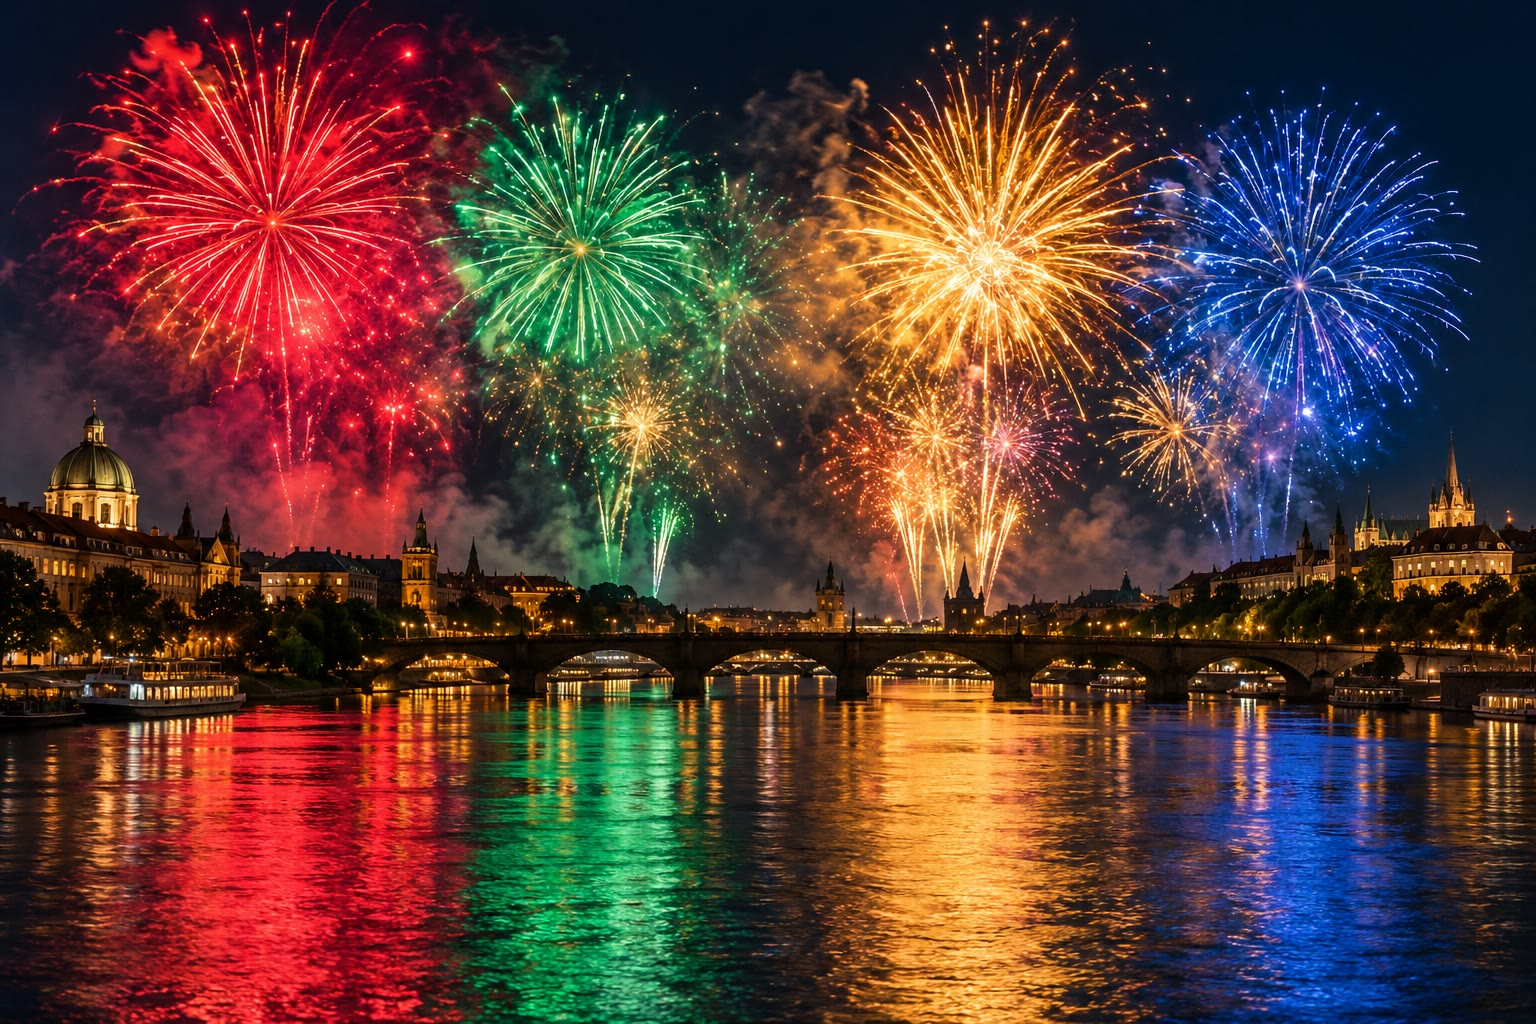
\includegraphics[width=0.58\linewidth]{images/book3/ai/b2-32-fireworks.jpg}

{\small Feu d'artifice au-dessus d'une rivière (illustration). Le jaune du sodium est la lumière de ses
atomes~; les rouges et les verts profonds viennent surtout de petites molécules de strontium et de baryum
formées dans la flamme.}
\end{omfigure}

\begin{recall}
Le volume scolaire~: isotopes et leurs abondances. Le volume de première année~: niveaux d'énergie et raies
spectrales, absorbance et loi de Beer--Lambert, carbocations et radicaux, nombre d'insaturations.
\Cref{ch:b2:chromatography}~: la \omterm{def:b2:chromatography:techniques}{chromatographie en phase gazeuse}, qui alimente souvent un spectromètre
de masse.
\end{recall}

\section{Le spectromètre de masse}

\begin{definition}[Spectrométrie de masse]\label{def:b2:mass-spec-atomic:spectrum}
La \emph{spectrométrie de masse}\index{spectrometrie de masse@spectrométrie de masse} transforme les
molécules d'un échantillon en ions gazeux, sépare les ions selon leur \emph{rapport masse sur charge}\index{rapport masse sur charge} $m/z$
(la masse en unités de masse atomique unifiée divisée par le nombre de charges) et les compte. Le
\emph{spectre de masse}\index{spectre de masse} représente l'abondance des ions en fonction de $m/z$, le
plus souvent en intensités relatives~; son pic le plus intense, fixé à 100, est le \emph{pic de base}\index{pic de base}.
\end{definition}

Un spectromètre comporte trois parties. La source fabrique les ions. En ionisation électronique (IE), la
vapeur de l'échantillon traverse un faisceau d'électrons de \qty{70}{eV}, qui arrachent un électron aux
molécules et leur laissent un excès d'énergie, si bien que beaucoup se brisent. En ionisation par
électronébulisation (ESI), une solution est pulvérisée à partir d'une aiguille chargée~; à mesure que les
gouttelettes s'évaporent, des molécules les quittent en portant un proton supplémentaire (ou un ion
sodium), intactes~: c'est la méthode de choix pour les grosses molécules fragiles. L'analyseur trie
ensuite les ions, et un détecteur les compte.

\begin{omfigure}
\begin{tikzpicture}[x=1cm, y=1cm]
\draw[black!70, fill=omDef!10, rounded corners=2pt] (0,-0.6) rectangle (1.6,0.6);
\node[font=\small, align=center] at (0.8,0) {source\\d'ions};
\draw[black!70] (2.0,-0.7) -- (2.0,0.7); \draw[black!70] (2.4,-0.7) -- (2.4,0.7);
\node[font=\footnotesize] at (2.2,1.0) {grilles, $U$};
\draw[black!70] (2.6,-0.5) rectangle (8.4,0.5);
\node[font=\small] at (5.6,0.8) {tube de vol sans champ, longueur $L$};
\draw[black!70, fill=black!15] (8.5,-0.6) rectangle (8.8,0.6);
\node[font=\small, align=center] at (9.6,0) {détecteur};
\foreach \x/\c in {3.4/omThm, 4.6/omDef, 6.3/omMeth}{\fill[\c] (\x,0) circle (0.1);}
\draw[->, thick] (6.6,0) -- (7.4,0);
\node[font=\footnotesize, align=center] at (5.5,-0.85) {les ions légers devancent les lourds};
\end{tikzpicture}
\par\vspace{4pt}

{\small Un analyseur à temps de vol (schéma). Des ions accélérés par la même différence de potentiel
$U$ partent avec la même énergie cinétique~; dans le tube de vol, les plus légers vont plus vite et
atteignent les premiers le détecteur.}
\end{omfigure}

\begin{proposition}[Temps de vol]\label{prop:b2:mass-spec-atomic:time-of-flight}
Un ion de masse $m$ et de charge $ze$, accéléré à partir du repos par une différence de potentiel $U$,
traverse un tube sans champ de longueur $L$ en
\begin{equation*}
t = L\sqrt{\frac{m}{2zeU}}:
\end{equation*}
le temps de vol croît comme la racine carrée de $m/z$.
\end{proposition}

\begin{proof}
La conservation de l'énergie dans le champ accélérateur donne $\tfrac12mv^2 = zeU$, donc $v = \sqrt{2zeU/m}$,
et le tube est traversé à vitesse constante~: $t = L/v$.
\end{proof}

D'autres analyseurs trient les ions autrement~: un quadripôle ne laisse passer que les ions d'un seul $m/z$
à la fois, sélectionnés par des tensions oscillantes appliquées à quatre barreaux~; un secteur magnétique
courbe les ions sur des cercles dont le rayon dépend de leur quantité de mouvement. Dans tous, seul $m/z$
est mesuré~; la plupart des ions formés par IE portent une seule charge, si bien que $m/z$ est simplement
leur masse.

\section{L'ion moléculaire}

\begin{definition}[Ions moléculaire et fragments]\label{def:b2:mass-spec-atomic:molecular-ion}
L'\emph{ion moléculaire}\index{ion moleculaire@ion moléculaire} $\mathrm M^{+\bullet}$ est le
radical-cation formé quand une molécule perd un électron~; son $m/z$ est la masse molaire de la molécule
formée des isotopes les plus abondants. Un \emph{ion fragment}\index{ion fragment} provient de l'ion
moléculaire par rupture de liaisons.
\end{definition}

L'\omterm{def:b2:mass-spec-atomic:molecular-ion}{ion moléculaire} donne la masse moléculaire, premier renseignement sur une inconnue. Il est parfois
faible ou absent en IE, quand l'\omterm{def:b2:mass-spec-atomic:molecular-ion}{ion moléculaire} se brise trop facilement~; l'électronébulisation, qui
donne $[\mathrm M +
\mathrm H]^+$ une unité plus haut, la confirme alors.

\begin{definition}[Règle de l'azote]\label{def:b2:mass-spec-atomic:nitrogen-rule}
La \emph{règle de l'azote}\index{regle de l'azote@règle de l'azote} énonce qu'une molécule a une masse
nominale impaire (la somme des nombres de masse de ses isotopes les plus abondants) si et seulement si
elle contient un nombre impair d'atomes d'azote.
\end{definition}

\begin{proposition}[Validité de la règle de l'azote]\label{prop:b2:mass-spec-atomic:nitrogen-rule}
La \omterm{def:b2:mass-spec-atomic:nitrogen-rule}{règle de l'azote} vaut pour toute molécule sans électron célibataire construite à partir de C, H, N,
O, S et des halogènes.
\end{proposition}

\begin{proof}
Les masses nominales sont paires pour C (12), N (14), O (16) et S (32), impaires pour H (1) et les
halogènes (19, 35, 79, 127). Les valences sont paires pour C, O et S, impaires pour H, N et les
halogènes. Dans une molécule sans électron célibataire, chaque liaison utilise une valence de chacun de
ses deux atomes, si bien que la somme de toutes les valences est paire, et le nombre d'atomes de valence
impaire, $n_{\ce{H}} + n_{\ce{X}} + n_{\ce{N}}$, est pair. La parité de la masse nominale est celle de
$n_{\ce{H}} + n_{\ce{X}}$, qui est donc celle de
$n_{\ce{N}}$.
\end{proof}

\begin{definition}[Massif isotopique]\label{def:b2:mass-spec-atomic:isotope-pattern}
Le \emph{massif isotopique}\index{massif isotopique} d'un ion est le groupe de pics en $M$, $M+1$,
$M+2$, \dots\ produits par les molécules contenant des isotopes plus lourds, avec des intensités
proportionnelles aux abondances de ces formes isotopiques.
\end{definition}

\begin{proposition}[Le pic $M+1$]\label{prop:b2:mass-spec-atomic:m-plus-one}
Pour un ion comportant $n_C$ atomes de carbone et aucun autre élément doté d'un isotope $+1$ notable,
\begin{equation*}
\frac{I(M+1)}{I(M)} \approx n_C\,\frac{a_{13}}{a_{12}} \approx n_C \times 1.1~\%,
\end{equation*}
où $a_{12} = 0.989$ et $a_{13} = 0.011$ sont les fractions molaires des deux isotopes du carbone.
% ledger: iso:C12, iso:C13
\end{proposition}

\begin{proof}
La probabilité que les $n_C$ carbones soient tous des \ce{^{12}C} vaut $a_{12}^{n_C}$~; que l'un d'eux
exactement soit un \ce{^{13}C}, $n_C\,a_{13}a_{12}^{n_C - 1}$ (loi binomiale). Le rapport vaut $n_C\,a_{13}/a_{12}$,
et les autres contributions (deux \ce{^{13}C}, \ce{^2H}, \ce{^{15}N}) sont plus petites d'un facteur de
l'ordre de $a_{13}$ ou moins.
\end{proof}

\begin{proposition}[Chlore et brome]\label{prop:b2:mass-spec-atomic:halogen-patterns}
Pour un ion comportant $p$ atomes de chlore et $q$ atomes de brome, les intensités de $M$, $M+2$, $M+4$,
\dots\ sont les coefficients du développement de $(a_{35} + a_{37}x)^p(a_{79} + a_{81}x)^q$ en puissances
de $x$, chaque puissance de $x$ représentant 2 unités de masse. Avec $a_{35} = 0.758$, $a_{37} = 0.242$,
$a_{79} = 0.5069$ et
$a_{81} = 0.4931$, un chlore donne $M : M+2 \approx 3 : 1$ et un brome $\approx 1 : 1$.
% ledger: iso:Cl35, iso:Cl37, iso:Br79, iso:Br81
\end{proposition}

\begin{proof}
Chaque atome d'halogène est, indépendamment des autres, l'isotope léger ou l'isotope lourd, qui ajoute 2
à la masse. La probabilité d'un nombre donné $j$ d'atomes lourds est le coefficient de $x^j$ dans le
produit d'un facteur par atome, c'est-à-dire le développement annoncé (la loi binomiale, élément par élément).
\end{proof}

\begin{omfigure}
\pgfplotsset{clu/.style={width=0.25\linewidth, height=3.3cm, ybar, bar width=5pt, ymin=0, ymax=118,
  xmin=-1.2, xmax=5.2, xtick={0,2,4}, xticklabels={$M$,$M\!+\!2$,$M\!+\!4$},
  tick label style={font=\tiny}, ytick=\empty, axis x line=bottom, axis y line=none,
  title style={font=\small, yshift=-4pt}, nodes near coords, nodes near coords style={font=\tiny},
  point meta=y, every node near coord/.append style={/pgf/number format/fixed, /pgf/number format/precision=0}}}
\begin{tikzpicture}
\begin{axis}[clu, title={Cl}]
\addplot[fill=omDef!55, draw=omDef, y filter/.expression={y==0 ? nan : y}] table[x=off, y=Cl] {figdata/out/bachelor-2-mass-spectra-a.dat};
\end{axis}
\end{tikzpicture}\hfill
\begin{tikzpicture}
\begin{axis}[clu, title={Cl$_2$}]
\addplot[fill=omDef!55, draw=omDef] table[x=off, y=Cl2] {figdata/out/bachelor-2-mass-spectra-a.dat};
\end{axis}
\end{tikzpicture}\hfill
\begin{tikzpicture}
\begin{axis}[clu, title={Br}]
\addplot[fill=omThm!45, draw=omThm, y filter/.expression={y==0 ? nan : y}] table[x=off, y=Br] {figdata/out/bachelor-2-mass-spectra-a.dat};
\end{axis}
\end{tikzpicture}\hfill
\begin{tikzpicture}
\begin{axis}[clu, title={Br$_2$}]
\addplot[fill=omThm!45, draw=omThm] table[x=off, y=Br2] {figdata/out/bachelor-2-mass-spectra-a.dat};
\end{axis}
\end{tikzpicture}\hfill
\begin{tikzpicture}
\begin{axis}[clu, title={ClBr}]
\addplot[fill=omMeth!45, draw=omMeth] table[x=off, y=ClBr] {figdata/out/bachelor-2-mass-spectra-a.dat};
\end{axis}
\end{tikzpicture}

{\small \omterm{def:b2:mass-spec-atomic:isotope-pattern}{Massifs isotopiques} d'ions contenant du chlore et du brome, calculés à partir des abondances
isotopiques (\cref{prop:b2:mass-spec-atomic:halogen-patterns})~; le pic le plus intense de chaque groupe
est fixé à 100. Ces massifs sont des empreintes~: 3 : 1 pour un chlore, 1 : 1 pour un brome, 1 : 2 : 1
pour deux bromes.}
% figdata: bachelor-2/mass-spectra.py part a
\end{omfigure}

\begin{definition}[Masse exacte]\label{def:b2:mass-spec-atomic:exact-mass}
La \emph{masse monoisotopique}\index{masse monoisotopique} d'un ion est la somme des masses exactes de
ses isotopes les plus abondants (\ce{^{12}C} = 12 exactement, \ce{^1H} = 1.007825, \ce{^{16}O} = 15.994915,
\ce{^{14}N} = 14.003074 u). La \emph{spectrométrie de masse à haute résolution}\index{spectrometrie de masse a haute resolution@spectrométrie de masse à haute résolution}
mesure $m/z$ à quelques millièmes d'unité près ou mieux, ce qui suffit à distinguer des ions de même
masse nominale mais de formules différentes.
% ledger: mass:C12, mass:H1, mass:O16, mass:N14
\end{definition}

\begin{proposition}[Pouvoir de résolution]\label{prop:b2:mass-spec-atomic:resolving}
Deux ions de masses $m$ et $m + \Delta m$ sont séparés par un analyseur de pouvoir de résolution au moins
égal à $R = m/\Delta m$. À la masse nominale 28, séparer \ce{CO+} (27.9949) de \ce{N2+} (28.0061) exige $R
\approx 2.5 \times 10^3$~; séparer \ce{N2+} de \ce{C2H4+} (28.0313), $R \approx 1.1 \times 10^3$.
\end{proposition}

\begin{proof}
Le pouvoir de résolution est défini comme $m/\Delta m$ pour le plus petit $\Delta m$ que l'analyseur
sépare. Les masses exactes découlent des masses isotopiques~: $12 + 15.994915$, $2 \times 14.003074$, $24 + 4 \times
1.007825$~; d'où $28/(28.0061 - 27.9949) \approx 2.5 \times 10^3$ et $28/(28.0313 - 28.0061) \approx
1.1 \times 10^3$.
\end{proof}

\section{Fragmentation}

L'\omterm{def:b2:mass-spec-atomic:molecular-ion}{ion moléculaire} formé par IE porte bien plus d'énergie qu'il n'en faut pour rompre n'importe quelle
liaison, et il se brise selon les voies qui donnent les produits les plus stables~: cations stabilisés,
petites molécules neutres stables ou radicaux. On lit les fragments comme des pertes à partir de $M$ (15
pour \ce{CH3}, 29 pour \ce{C2H5} ou \ce{CHO}, 18
pour l'eau, 28 pour CO ou l'éthène) et comme des ions caractéristiques.

\begin{definition}[Deux fragmentations]\label{def:b2:mass-spec-atomic:fragmentation}
Dans une \emph{coupure $\alpha$}\index{coupure alpha@coupure $\alpha$}, une liaison du carbone voisin d'un
hétéroatome ou d'un carbonyle se rompt, en laissant un cation stabilisé par le doublet de l'hétéroatome
(un \omterm{def:b2:aromatic-substitution:friedel-crafts}{ion acylium} $\mathrm{R{-}C{\equiv}O^+}$ pour une cétone, un ion iminium pour une amine). Le
\emph{réarrangement de McLafferty}\index{rearrangement de McLafferty@réarrangement de McLafferty} d'un
composé carbonylé transfère un hydrogène du carbone
$\gamma$ à l'oxygène du carbonyle et rompt la liaison $\alpha$--$\beta$, en libérant un alcène et un
radical-cation d'\omterm{def:b2:enolates-aldol:tautomerism}{énol}.
\end{definition}

\begin{omfigure}
\begin{tikzpicture}
\begin{axis}[width=0.48\linewidth, height=4.6cm, xmin=10, xmax=80, ymin=0, ymax=118,
  xlabel={$m/z$}, ylabel={intensité relative}, label style={font=\small}, tick label style={font=\scriptsize},
  title={\small butan-2-one}, ycomb, xtick={15,29,43,57,72}]
\addplot[omDef, thick] table[x=mz, y=I] {figdata/out/bachelor-2-mass-spectra-b.dat};
\node[font=\tiny, anchor=south] at (axis cs:43,100) {43};
\node[font=\tiny, anchor=south] at (axis cs:72,25) {72};
\node[font=\tiny, anchor=south] at (axis cs:57,8) {57};
\node[font=\tiny, anchor=south] at (axis cs:29,17) {29};
\end{axis}
\end{tikzpicture}\hfill
\begin{tikzpicture}
\begin{axis}[width=0.48\linewidth, height=4.6cm, xmin=10, xmax=140, ymin=0, ymax=118,
  xlabel={$m/z$}, ylabel={intensité relative}, label style={font=\small}, tick label style={font=\scriptsize},
  title={\small 1-bromopropane}, ycomb, xtick={27,43,79,107,122}]
\addplot[omThm, thick] table[x=mz, y=I] {figdata/out/bachelor-2-mass-spectra-c.dat};
\node[font=\tiny, anchor=south] at (axis cs:43,100) {43};
\node[font=\tiny, anchor=south] at (axis cs:123,9) {122, 124};
\node[font=\tiny, anchor=south] at (axis cs:27,26) {27};
\node[font=\tiny, anchor=south east] at (axis cs:40.5,31) {41};
\end{axis}
\end{tikzpicture}

{\small Spectres d'ionisation électronique (données du NIST WebBook). Butan-2-one~: \omterm{def:b2:mass-spec-atomic:molecular-ion}{ion moléculaire} à 72~;
les coupures $\alpha$ donnent les \omterm{def:b2:aromatic-substitution:friedel-crafts}{ions acylium} \ce{CH3CO+} (43, \omterm{def:b2:mass-spec-atomic:spectrum}{pic de base}) et \ce{C2H5CO+} (57).
1-bromopropane~: l'\omterm{def:b2:mass-spec-atomic:molecular-ion}{ion moléculaire} est une paire 1 : 1 à 122 et 124 (\ce{^{79}Br}, \ce{^{81}Br})~; la perte
de l'atome de brome laisse \ce{C3H7+} à 43, le \omterm{def:b2:mass-spec-atomic:spectrum}{pic de base}.}
% figdata: bachelor-2/mass-spectra.py parts b, c
% ledger: ms:butanone, ms:bromopropane
\end{omfigure}

\begin{omfigure}
\setchemfig{atom sep=1.8em}
\schemestart
\chemfig{[:-30]\chemabove{O}{\scriptstyle +\bullet}?[a]=[:-90]C(-[:-150]H_3C)-[:-30]CH_2-[:30]CH_2-[:90]CH_2-[:150]H?[a,1,{dash pattern=on 1pt off 1.5pt}]}
\arrow{->}[,1.0]
\chemfig{CH_2=C(-[2]OH)-CH_3}\,$^{+\bullet}$
\+
\chemfig{CH_2=CH_2}
\schemestop
\par\vspace{6pt}

{\small Le \omterm{def:b2:mass-spec-atomic:fragmentation}{réarrangement de McLafferty} de la pentan-2-one, dessiné par son arrangement cyclique à six
atomes~: l'hydrogène du carbone $\gamma$ passe sur l'oxygène, la liaison $\alpha$--$\beta$ se rompt,
l'éthène part, et le radical-cation de l'\omterm{def:b2:enolates-aldol:tautomerism}{énol} de la propanone reste à $m/z$ 58.}
\end{omfigure}

\begin{proposition}[Condition de McLafferty]\label{prop:b2:mass-spec-atomic:mclafferty}
Un \omterm{def:b2:mass-spec-atomic:fragmentation}{réarrangement de McLafferty} exige un hydrogène sur le carbone $\gamma$. Il libère un alcène et laisse
un radical-cation dont la masse a la parité de la masse moléculaire (paire pour un composé sans azote).
\end{proposition}

\begin{proof}[Argument]
L'hydrogène est transféré par un arrangement cyclique à six atomes formé de l'oxygène, du carbone du
carbonyle, des carbones $\alpha$, $\beta$ et $\gamma$ et de l'hydrogène lui-même~: seul un hydrogène
$\gamma$ atteint l'oxygène sans tension. L'ion formé conserve le groupe carbonyle, le carbone $\alpha$ et
l'hydrogène transféré~; ce qui part est un alcène, molécule neutre de masse paire, si bien que l'ion
conserve la parité de $M$, ce qui le distingue des cations de masse impaire formés par les coupures simples.
\end{proof}

\begin{method}[Lire un spectre de masse]\label{met:b2:mass-spec-atomic:read-ms}
\begin{enumerate}
  \item Repérer l'\omterm{def:b2:mass-spec-atomic:molecular-ion}{ion moléculaire} (le $m/z$ le plus élevé du massif principal, avec des pertes plausibles au-dessous).
  \item Lire son \omterm{def:b2:mass-spec-atomic:isotope-pattern}{massif isotopique}~: Cl, Br, S~; le pic $M+1$ donne le nombre de carbones.
  \item Appliquer la \omterm{def:b2:mass-spec-atomic:nitrogen-rule}{règle de l'azote}~; proposer des formules et leur nombre d'insaturations.
  \item Lire les pertes à partir de $M$ et les ions caractéristiques (43 \ce{CH3CO+} ou \ce{C3H7+}, 77
        \ce{C6H5+}, 91 \ce{C7H7+}, 105 \ce{C6H5CO+})~; chercher des ions de McLafferty de masse paire.
  \item Proposer des structures~; vérifier que chaque pic important est expliqué.
\end{enumerate}
\end{method}

\section{Spectroscopie atomique}

Les atomes n'ont ni vibrations ni rotations~; leurs spectres sont des raies fines, une par transition entre
niveaux électroniques, à des longueurs d'onde caractéristiques de l'élément. Le jaune d'une flamme au
sodium est le doublet de raies à \qty{589.0}{nm} et \qty{589.6}{nm}~; le rouge carmin du lithium, une raie
à \qty{670.8}{nm}~;
la raie la plus intense des atomes de strontium se trouve à \qty{460.7}{nm} et celle des ions baryum à
\qty{455.4}{nm}, dans le bleu~: les rouges et les verts des feux d'artifice viennent surtout de molécules
de ces métaux, et non de leurs atomes.
% ledger: asd:NaD2, asd:NaD1, asd:Li671, asd:Sr461, asd:Ba455

\begin{definition}[Spectrométries atomiques]\label{def:b2:mass-spec-atomic:atomic}
En \emph{spectrométrie d'émission atomique}\index{spectrometrie d'emission atomique@spectrométrie d'émission atomique},
l'échantillon est atomisé et excité dans une flamme ou un plasma, et l'on mesure l'intensité d'une raie
d'émission de l'élément. En \emph{spectrométrie d'absorption atomique}\index{spectrometrie d'absorption atomique@spectrométrie d'absorption atomique}
(SAA), l'échantillon est atomisé dans une flamme ou un four en graphite et l'on mesure l'absorbance des
atomes à une raie de résonance, émise par une \emph{lampe à cathode creuse}\index{lampe a cathode creuse@lampe à cathode creuse}
dont la cathode est faite de l'élément lui-même. Dans un \emph{plasma à couplage inductif}\index{plasma a couplage inductif@plasma à couplage inductif}
(ICP), de l'argon chauffé par un champ de radiofréquence à plusieurs milliers de kelvins atomise et
ionise l'échantillon~; le plasma alimente un spectromètre d'émission (ICP-OES) ou un spectromètre de
masse (ICP-MS).
\end{definition}

\begin{omfigure}
\begin{tikzpicture}[x=1cm, y=1cm, box/.style={draw=black!70, rounded corners=2pt, fill=white,
  font=\small, align=center, minimum height=0.8cm, inner sep=3pt}]
\node[box] (lamp) at (0,0) {lampe à cathode\\creuse (Cu)};
\shade[top color=omThm!60, bottom color=omThm!10] (2.6,-0.25) -- (3.3,-0.25) -- (3.15,0.75) -- (2.75,0.75) -- cycle;
\draw[black!70, fill=black!15] (2.4,-0.45) rectangle (3.5,-0.25);
\node[font=\footnotesize] at (2.95,-0.75) {flamme (atomes)};
\node[box] (mono) at (6.1,0) {mono-\\chromateur};
\node[box] (det) at (8.5,0) {détecteur};
\node[box] (data) at (10.8,0) {absorbance};
\draw[->, thick, omDef] (lamp.east) -- (mono.west);
\draw[->, thick] (mono) -- (det); \draw[->, thick] (det) -- (data);
\node[font=\footnotesize, omDef] at (4.4,0.3) {$I_0 \to I$};
\end{tikzpicture}
\par\vspace{4pt}

{\small Un spectromètre d'absorption atomique (schéma). La lampe émet les raies du cuivre lui-même, dont
la raie de résonance à \qty{324.75}{nm}~; les atomes de cuivre de la flamme l'absorbent, et le
monochromateur isole cette raie pour le détecteur.}
% ledger: asd:Cu325
\end{omfigure}

\begin{proposition}[L'absorption atomique est quantitative]\label{prop:b2:mass-spec-atomic:aas}
Sur un domaine de concentrations, l'absorbance mesurée à une raie de résonance est proportionnelle à la
concentration de l'élément dans la solution pulvérisée dans la flamme.
\end{proposition}

\admitted

C'est la loi de Beer--Lambert du volume de première année appliquée à des atomes libres~: la flamme
transforme en atomes une fraction constante de la solution, et la raie de la lampe, plus étroite que la
raie d'absorption, se comporte comme une lumière monochromatique. À forte concentration, la raie sature et
la courbe d'étalonnage s'incurve, d'où la vérification du domaine de travail.

\begin{method}[Étalonner une mesure d'absorption atomique]\label{met:b2:mass-spec-atomic:aas-calibration}
\begin{enumerate}
  \item Préparer un blanc et quatre ou cinq étalons couvrant le domaine attendu, dans la même matrice
        acide que les échantillons.
  \item Mesurer leurs absorbances à la raie choisie~; ajuster $A = a\,c$ (ou $A = a\,c + b$)~; vérifier la
        linéarité.
  \item Mesurer les échantillons, dilués si nécessaire pour tomber dans le domaine~; calculer $c = (A - b)/a$.
  \item Mesurer de nouveau un étalon à la fin pour contrôler la dérive~; tenir compte de chaque dilution.
\end{enumerate}
\end{method}

L'ICP-MS atteint les plus basses concentrations, mais ses ions peuvent coïncider en masse avec d'autres de
même masse nominale~: \ce{^{40}Ar^{16}O+}, issu du gaz plasmagène, tombe sur \ce{^{56}Fe+}, et
\ce{^{40}Ar+} sur
\ce{^{40}Ca+}. Un analyseur à haute résolution, une cellule de collision ou un autre isotope de l'analyte
supprime l'interférence. Les limites de détection, et la façon de les mesurer, font l'objet du
\cref{ch:b2:measurement-statistics}.

\begin{history}[Peser les atomes, voir les éléments]
\begin{minipage}[t]{0.17\linewidth}
\vspace{0pt}
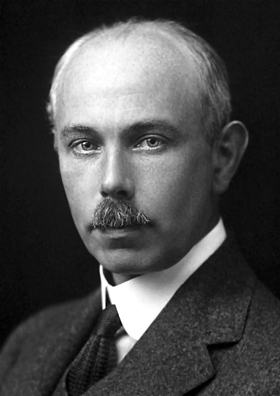
\includegraphics[width=\linewidth]{images/book3/aston.jpg}
\end{minipage}\hspace{0.02\linewidth}%
\begin{minipage}[t]{0.24\linewidth}
\vspace{0pt}
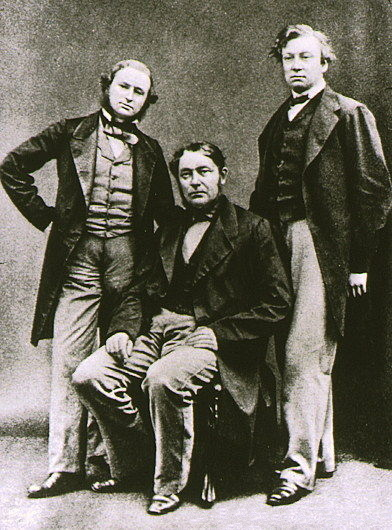
\includegraphics[width=\linewidth]{images/book3/kirchhoff-bunsen.jpg}
\end{minipage}\hfill
\begin{minipage}[t]{0.54\linewidth}
\vspace{0pt}
Gustav Kirchhoff et Robert Bunsen montrèrent vers 1860 que chaque élément donne ses propres raies dans
une flamme, et découvrirent le césium et le rubidium grâce à des raies inconnues. Le spectrographe de
masse de Francis Aston, à partir de 1919, montra que la plupart des éléments sont des mélanges
d'isotopes~; il reçut le prix Nobel de chimie 1922. (Photographies~: Aston, auteur inconnu, domaine
public~; Kirchhoff, Bunsen et Henry Roscoe en 1862, collection de Roscoe, domaine public~; Wikimedia Commons.)
\end{minipage}
\end{history}

\section{Exercices}

\begin{exercise}[$\star$]\label{exo:b2:mass-spec-atomic:1}
Donner le $m/z$~: de l'\omterm{def:b2:mass-spec-atomic:molecular-ion}{ion moléculaire} du benzène \ce{C6H6}~; d'un ion de masse \qty{400}{u} portant deux
charges~; de la molécule protonée de caféine (\ce{C8H10N4O2}, masse nominale 194) formée par
électronébulisation.
\end{exercise}

\begin{exercise}[$\star$]\label{exo:b2:mass-spec-atomic:2}
Un composé formé de C, H, N et O a un \omterm{def:b2:mass-spec-atomic:molecular-ion}{ion moléculaire} à $m/z$ 73. Que peut-on dire de ses atomes
d'azote~? Proposer une formule.
\end{exercise}

\begin{exercise}[$\star$]\label{exo:b2:mass-spec-atomic:3}
Un massif d'\omterm{def:b2:mass-spec-atomic:molecular-ion}{ion moléculaire} montre deux pics distants de deux unités, de hauteurs presque égales. Un autre
montre deux pics distants de deux unités, dans le rapport 3 : 1. Quels halogènes~?
\end{exercise}

\begin{exercise}[$\star$]\label{exo:b2:mass-spec-atomic:4}
Un sel colore une flamme en jaune~; un autre en rouge carmin. Identifier les éléments et donner les
longueurs d'onde de leurs raies.
\end{exercise}

\begin{exercise}[$\star\star$]\label{exo:b2:mass-spec-atomic:5}
Un hydrocarbure présente $M$ à 100~\% et $M+1$ à 6.7~\%. Combien d'atomes de carbone contient-il~?
\end{exercise}

\begin{exercise}[$\star\star$]\label{exo:b2:mass-spec-atomic:6}
Calculer les masses exactes de \ce{CO}, \ce{N2} et \ce{C2H4} et le pouvoir de résolution nécessaire pour
séparer chaque paire.
\end{exercise}

\begin{exercise}[$\star\star$]\label{exo:b2:mass-spec-atomic:7}
Le spectre IE de la pentan-3-one présente des pics à 86, 57 (\omterm{def:b2:mass-spec-atomic:spectrum}{pic de base}) et 29. Les attribuer.
\end{exercise}

\begin{exercise}[$\star\star$]\label{exo:b2:mass-spec-atomic:8}
Le spectre de la pentan-2-one présente des pics à 86, 71, 58 et 43 (\omterm{def:b2:mass-spec-atomic:spectrum}{pic de base}). Les attribuer, et
expliquer pourquoi la pentan-3-one ne présente qu'un petit pic à 58.
\end{exercise}

\begin{exercise}[$\star\star$]\label{exo:b2:mass-spec-atomic:9}
Des étalons de cuivre à 1.0, 2.0, 3.0 et \qty{4.0}{mg/L} donnent les absorbances 0.052, 0.104, 0.155 et
0.207~; un échantillon donne 0.128 (données de l'exercice). Calculer sa concentration en cuivre.
\end{exercise}

\begin{exercise}[$\star\star\star$]\label{exo:b2:mass-spec-atomic:10}
Dans un analyseur à temps de vol, $L = \qty{1.00}{m}$ et $U = \qty{20.0}{kV}$. Calculer le temps de vol
d'un ion monochargé de masse \qty{1000}{u}, et l'intervalle de temps qui le sépare d'un ion de \qty{1001}{u}.
\end{exercise}

\begin{exercise}[$\star\star\star$]\label{exo:b2:mass-spec-atomic:11}
Calculer le massif de l'\omterm{def:b2:mass-spec-atomic:molecular-ion}{ion moléculaire} du dichlorométhane, \ce{CH2Cl2}~: valeurs de $m/z$ et intensités
relatives.
\end{exercise}

\begin{exercise}[$\star\star\star$]\label{exo:b2:mass-spec-atomic:12}
En ICP-MS, \ce{^{40}Ar^{16}O+} interfère avec \ce{^{56}Fe+}. Calculer le pouvoir de résolution nécessaire
pour les séparer, et proposer une autre solution.
\end{exercise}

\section{Problème~: un halogénure inconnu}

\begin{problem}[{Problème du week-end --- un massif d'ion moléculaire avec du chlore et du brome, le
nombre de carbones, les fragments, et une structure confrontée à chaque pic}]
\label{pb:b2:mass-spec-atomic:1}
Un liquide incolore, élué en un seul pic en \omterm{def:b2:chromatography:techniques}{chromatographie en phase gazeuse}, donne le \omterm{def:b2:mass-spec-atomic:spectrum}{spectre de masse} IE
ci-dessous (données du NIST WebBook). Pics principaux ($m/z$~: intensité relative)~: 156~: 14.5~;
157~: 0.5~; 158~: 18.6~; 159~: 0.6~; 160~: 4.4~; 107~: 6.7~; 109~: 6.3~; 93~: 3.3~; 95~: 2.9~; 77~: 59~;
79~: 18.7~; 76~: 39.5~; 49~: 12.9~; 51~: 4.3~; 41~: 100~; 39~: 26.2~; 27~: 24.6. Abondances isotopiques~:
\ce{^{35}Cl} 0.758, \ce{^{37}Cl} 0.242, \ce{^{79}Br} 0.5069,
\ce{^{81}Br} 0.4931, \ce{^{12}C} 0.989, \ce{^{13}C} 0.011.
% ledger: ms:bromochloropropane, iso:Cl35, iso:Cl37, iso:Br79, iso:Br81, iso:C12, iso:C13, mass:C12, mass:H1, mass:Br79, mass:Cl35

\begin{center}
\begin{tikzpicture}
\begin{axis}[width=0.8\linewidth, height=4.6cm, xmin=20, xmax=170, ymin=0, ymax=112,
  xlabel={$m/z$}, ylabel={intensité relative}, label style={font=\small},
  tick label style={font=\scriptsize}, ycomb, xtick={27,41,49,77,93,107,122,156}]
\addplot[omDef, thick] table[x=mz, y=I] {figdata/out/bachelor-2-mass-spectra-d.dat};
\end{axis}
\end{tikzpicture}
\end{center}
% figdata: bachelor-2/mass-spectra.py part d

\medskip
\noindent\textbf{Partie I --- L'\omterm{def:b2:mass-spec-atomic:molecular-ion}{ion moléculaire}.}
\begin{enumerate}
  \item Quels pics forment le massif de l'\omterm{def:b2:mass-spec-atomic:molecular-ion}{ion moléculaire}~? Pourquoi n'est-ce pas un pic unique~?
  \item Quels halogènes un massif de trois pics espacés de 2 suggère-t-il~?
  \item Quelle est la masse nominale de la forme isotopique la plus légère~?
  \item Que dit la \omterm{def:b2:mass-spec-atomic:nitrogen-rule}{règle de l'azote}~?
  \item Retrancher un \ce{^{79}Br} et un \ce{^{35}Cl}~: que reste-t-il, et quel fragment hydrocarboné a cette
        masse~?
  \item Proposer une formule brute et donner son nombre d'insaturations.
\end{enumerate}

\medskip
\noindent\textbf{Partie II --- Carbones et masse exacte.}
\begin{enumerate}[resume]
  \item À partir du rapport 157/156, estimer le nombre de carbones.
  \item Pourquoi cette estimation est-elle ici grossière~?
  \item Quelles formes isotopiques contribuent au pic à 158~?
  \item Calculer la \omterm{def:b2:mass-spec-atomic:exact-mass}{masse monoisotopique} de l'\omterm{def:b2:mass-spec-atomic:molecular-ion}{ion moléculaire}.
  \item \ce{C10H20O} a aussi la masse nominale 156 (exacte 156.151). Quel pouvoir de résolution sépare les
        deux~?
  \item L'\omterm{def:b2:mass-spec-atomic:molecular-ion}{ion moléculaire} d'un composé possédant une liaison C=C et les mêmes halogènes aurait-il une
        masse nominale différente~?
\end{enumerate}

\medskip
\noindent\textbf{Partie III --- Fragments.}
\begin{enumerate}[resume]
  \item La paire 77/79 est dans le rapport 3 : 1. Quel atome a été perdu, et quel est l'ion~?
  \item Expliquer le pic à 76.
  \item Attribuer le \omterm{def:b2:mass-spec-atomic:spectrum}{pic de base} à 41.
  \item Attribuer la paire 49/51.
  \item Attribuer les paires 93/95 et 107/109.
  \item Pourquoi un atome de brome se perd-il plus facilement qu'un atome de chlore~?
  \item Le 1-bromo-1-chloropropane donnerait \ce{CHBrCl+} à 127, 129 et 131. Le spectre l'appuie-t-il~?
\end{enumerate}

\medskip
\noindent\textbf{Partie IV --- La structure.}
\begin{enumerate}[resume]
  \item Proposer la structure.
  \item Vérifier qu'elle explique chacun des pics listés.
  \item Un \omterm{def:b2:mass-spec-atomic:fragmentation}{réarrangement de McLafferty} peut-il se produire~? Pourquoi~?
  \item Représenter l'isomère qui donnerait un pic intense à $m/z$ 63/65 et aucun à 49/51.
  \item Quelles formes isotopiques forment le pic à 160~?
  \item À partir des abondances isotopiques, calculer le rapport des pics $M$, $M+2$ et $M+4$ pour un
        chlore et un brome, et le comparer au spectre.
\end{enumerate}
\end{problem}
